%%%%%%%%%%%%%%%%%%%%%%%%%%%%%%%%%%%
\subsection{Purity Monitors} 
\label{sec:fdsp-slow-cryo-purity-mon}
%Laura, Jianming
A fundamental requirement of a LAr TPC is to make ionization electrons drift over long distances in LAr. Part of the charge is inevitably lost due to the presence of electronegative impurities in the liquid. To keep such loss to a minimum, purifying the LAr during operation is essential, as is the monitoring of impurities.

Residual gas analyzers are an obvious choice when analyzing gas argon and can be exploited for the monitoring of the gas in the ullage of the tank. Unfortunately, commercially available mass spectrometers have a detection limit of \SI{\sim10}{ppb}, whereas DUNE requires a sensitivity down to the \si{ppt} level. This gives us a case to construct small, ``portable'' devices, called ``purity monitors'', to monitor purity in all the phases of operations, guaranteeing successful commissioning and meeting the requirement to measure position-dependent purity necessary to achieve DUNE's physics goal. 
%Purity monitors also have the potential to be developed as a calibration tool that provides high precision and real-time electron lifetime measurements for wire-by-wire detector calibration. 

Purity monitors will be placed inside the cryostat, but outside of the detector TPC, as well as outside the cryostat within the recirculation system before and after filtration.

Purity monitors have been successfully deployed in the ICARUS detector and in the 35-ton prototype detector at Fermilab. The ProtoDUNE-SP and DP detectors will also employ purity monitors based on the same design principles used in the past. The ProtoDune-SP detector will utilize a string of purity monitors similar to that of the 35-ton detector, enabling measurement of the electron drift lifetime as a function of height.  A similar system design will be exploited in the DUNE FD, with modifications made to accommodate the instrumentation port placement relative to the purity monitor system and the requirements and constraints coming from the different geometric relations between the TPC and cryostat. 

\subsubsection{Physics and Simulation}
% Andrew, Jianming
A purity monitor is a miniature TPC which directly measures the electron lifetime, $\tau$, in the LAr and does not depend on the LAr TPC high voltage, electronics, and data acquisition. The concentration of electronegative impurities such as $\text{O}_2$ and $\text{H}_2\text{O}$ (which the electron lifetime mostly depends on) is inversely proportional to the electron lifetime according to the following formula~\cite{BakaleSowadaSchmidt}:

$$\tau = \sum_i \frac{1}{k_i [S_i]}$$

where the sum runs over all species of impurities in the liquid; $\tau$ is in s; $k_i$ is the electron attachment coefficient rate specific to the impurity in units of $l/(mol~s)$; and $[S_i]$ is the concentration of the specific impurity in units of $mol/l$. The electron attachment rate is a function of the electric field, but this field dependence is not significant for the range of LArTPC operation (electric field of \SI{500}{\volt\per\centi\meter}), as shown in Figure~\ref{fig:ks}. 

%\begin{figure}[h]
%\centering
%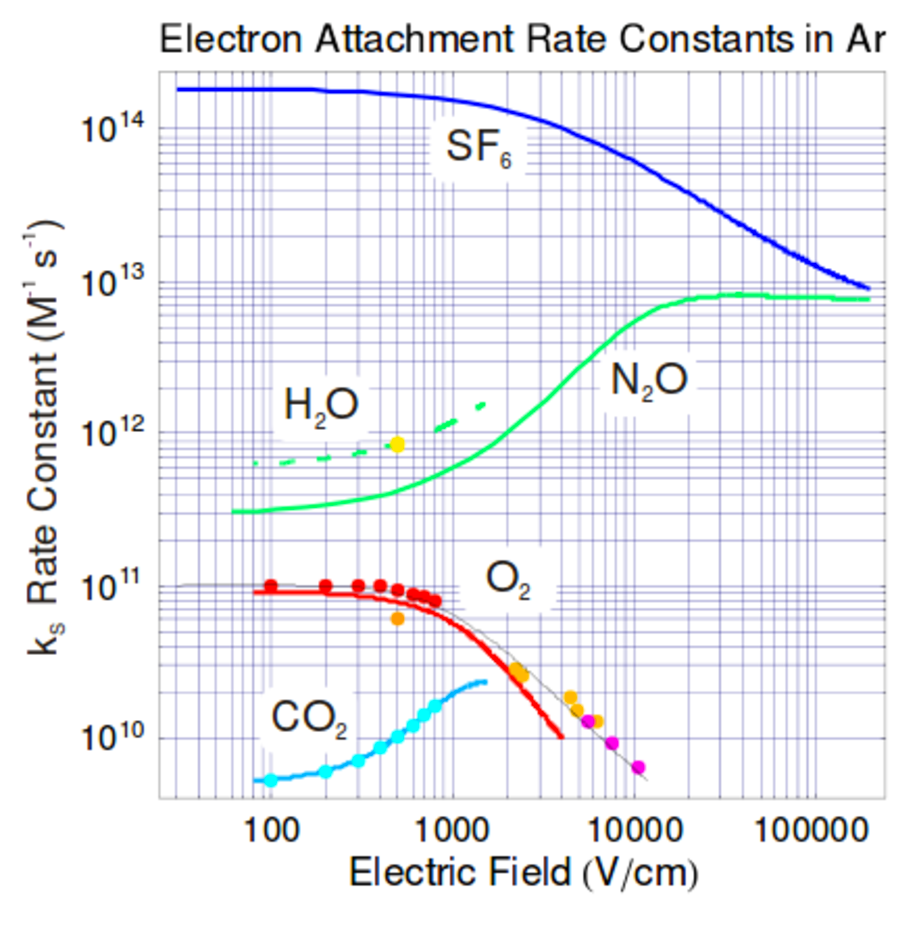
\includegraphics[height=6cm]{PrMon_ks.pdf}
%\caption{Electron attachment rate ($k_s$) as a function of electric field for several contaminants in a LAr TPC.}%Does this figure also need a citation, or is it something that one of us made specifically for this purpose?
%\label{fig:ks}
%\end{figure}
\begin{dunefigure}[Purity Monitor $k_s$]{fig:ks}
  {Electron attachment rate ($k_s$) as a function of electric field for several contaminants in a LAr TPC.}
  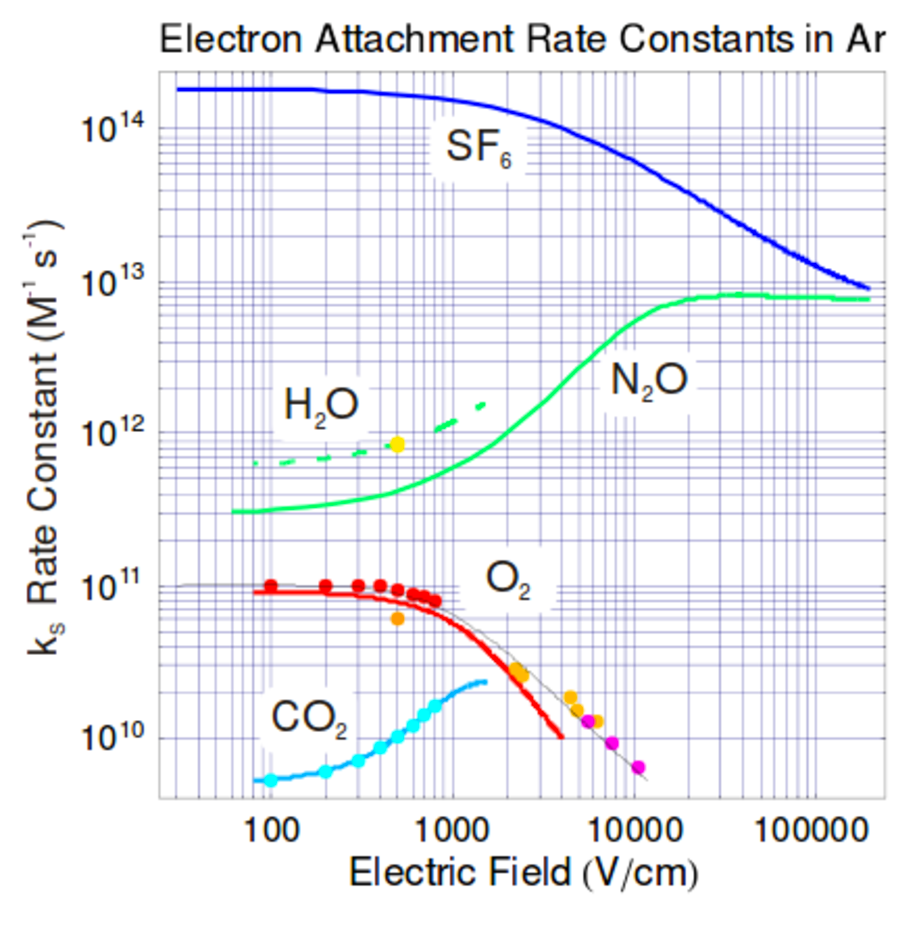
\includegraphics[width=0.4\textwidth]{PrMon_ks.pdf}%
\end{dunefigure}

Assuming all impurities affecting the electron lifetime are $\text{O}_2$, the electron lifetime is converted into the concentration of $\text{O}_2$ in \si{ppb} using the following:

$$ \text{O}_2 [\text{ppb}] = \frac{300 [\text{ppb}~\mu \text{s}]}{\tau [\mu \text{s}]}$$

Depending on their length and the electric field operated at, purity monitors can be sensitive to $\text{O}_2$ concentrations down to tens of \si{ppt}. 

The electron loss can be parameterized as

$$N(t) = N(0)e^{-t/\tau},$$

where $N(0)$ is the number of electrons generated by ionization, $N(t)$ is the number of electrons after drift time $t$, and $\tau$ is the electron lifetime. 

%For the single-phase DUNE far detector module the drift distance is \SI{3.6}{\meter}. For the dual-phase DUNE far detector module the maximum drift distance is \SI{12}{\meter}, and the requirement for the electron lifetime is even higher.   
For the DUNE single-phase far detector module, the drift distance is \SI{3.6}{\meter} and the electric field is \SI{500}{\volt\per\centi\meter}, giving a maximum drift time of \SI{\sim2.4}{\milli\second}. If the LAr TPC signal attenuation, [N(0)-N(t)]/N(0), is to be kept less than \SI{20}{\percent} over the entire drift distance, the necessary electron lifetime is $2.4/[-\ln(0.8)] \simeq 11 $ ms, and the corresponding LAr purity requirement is about \SI{30}{ppt}. For the DUNE dual-phase far detector module, the maximum drift distance is \SI{12}{\meter} and so the requirement on the electron lifetime is much higher. Furthermore, to best understand the LAr TPC detector response and performance, precise measurements of electron lifetime in LAr are very important and with purity monitors that can measure purity with high precision at specific points, it is possible to determine the gradient of the purity.

The DUNE 35-ton prototype detector at Fermilab was instrumented with four purity monitors. The data taken with them during the first part of the second phase is shown in Fig.~\ref{fig-35t-prm} and clearly shows the ability to measure the electron lifetime between \SI{100}{\micro\second} and \SI{3.5}{\milli\second}.  Because the scale of the DUNE far detectors are so large, the risk that sudden changes in the purity of the LAr being injected back into the cryostat might go unnoticed needs to be taken seriously.  If this were to occur for too long it would cause irreversible contamination to the LAr and terminate useful data taking.  Having purity monitors continuously monitoring the detector, placed in strategic places and then used as an interlock, it could be possible to salvage the overall purity of the detector and maintain the ability to take good data. An irreversible contamination cannot be tolerated in the DUNE far detectors, and so strategically placed purity monitors must be implemented to mitigate this risk. 

%\begin{figure}[t!]
%\begin{center}
%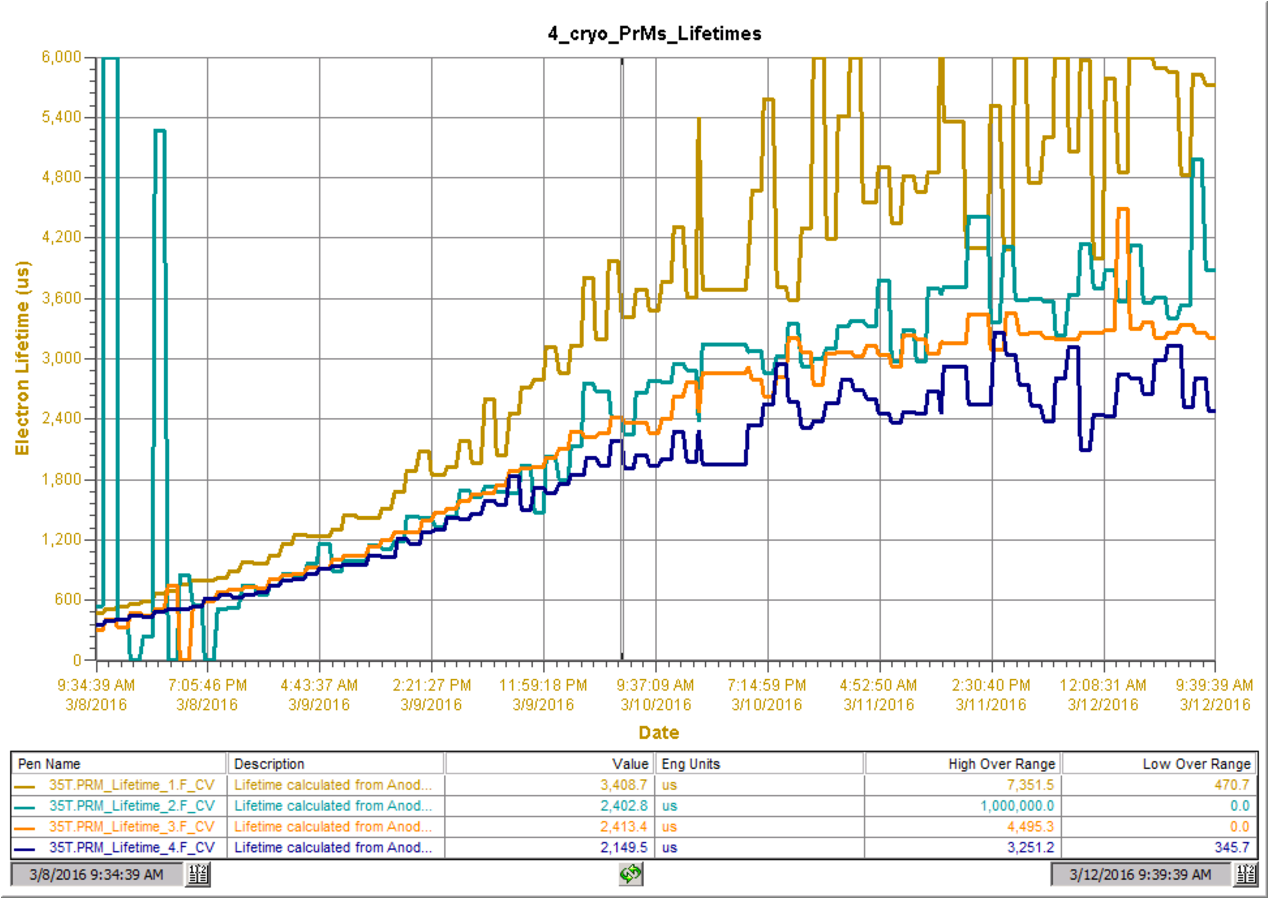
\includegraphics[width=10cm]{PrMon_35t-PrM.pdf}
%\caption{The measured electron lifetimes in the four purity monitors as a function of time at Fermilab 35T prototype.} \label{fig-35t-prm}
%\end{center}
%\end{figure}
\begin{dunefigure}[Purity Monitor lf]{fig-35t-prm}
  {The measured electron lifetimes in the four purity monitors as a function of time at Fermilab 35\si{t} prototype.}
  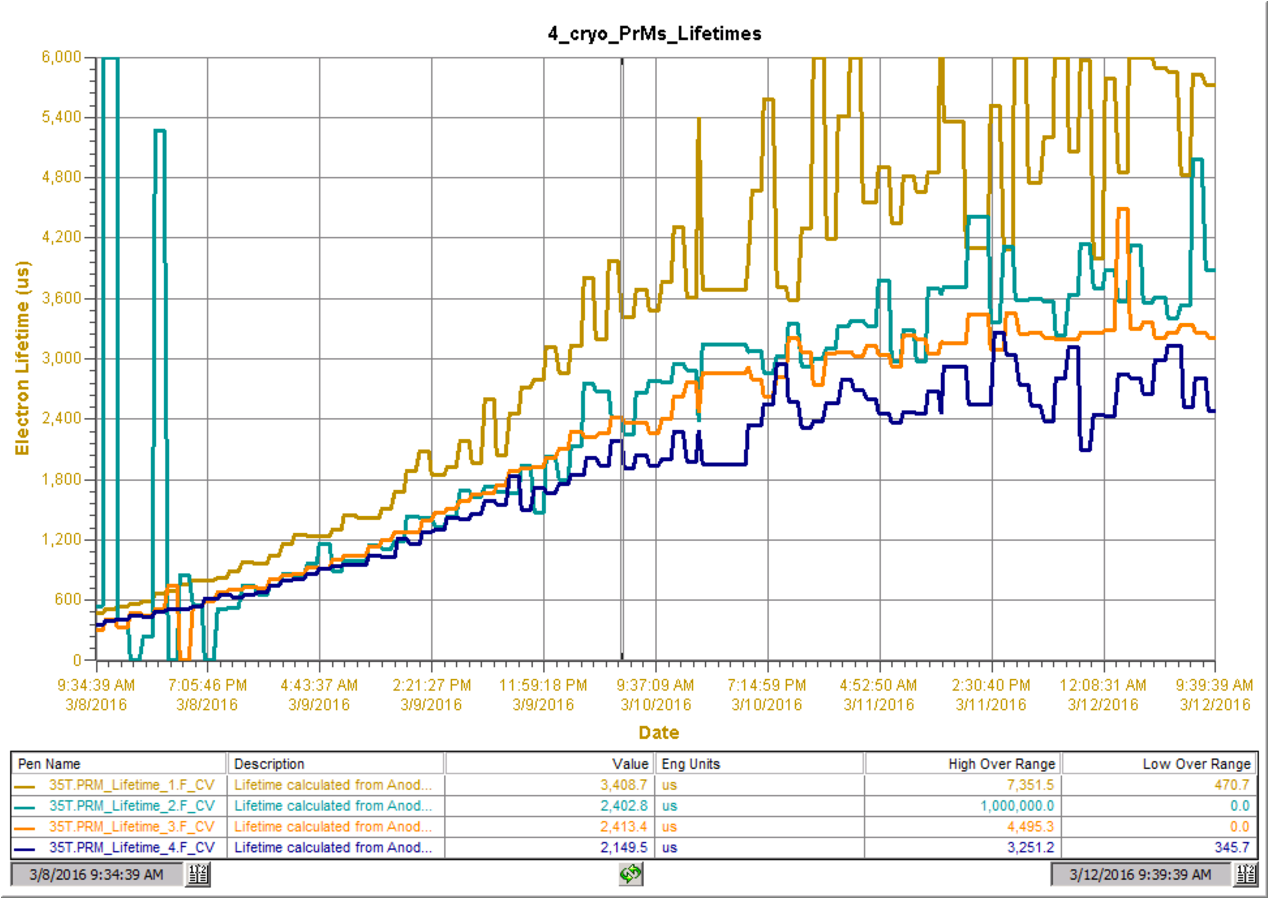
\includegraphics[width=0.4\textwidth]{PrMon_35t-PrM.pdf}%  
\end{dunefigure}


\subsubsection{Purity Monitor Design}
%Laura, Jianming
%WIP IF YOU HAVE MIP PARTICLES LIKE MUONS... NOT TRUE WHEN YOU ARE UNDERGROUND. ALSO, WE HAVE SEEN IN THE 311 THAT MUONS DO NOT DEPOSIT THE EXACT SAME AMOUNT OF ENERGY ACROSS THE TRACK 
%While the LAr TPC itself can measure the purity of the liquid argon based on the drift electron lifetime, this can only be done once a certain level of purity has been achieved, and until then it may be unclear what the level of purity is and if conditions in the detector are becoming better or worse. 

The basic design of a purity monitor is based on those used by the ICARUS experiment (Figure~\ref{fig:prm})\cite{Adamowski:2014daa}. It is a double-gridded ion chamber immersed in the liquid argon volume.   The purity monitor consists of four parallel, circular electrodes: a disk holding a photocathode, two grid rings (anode and cathode), and an anode disk. The cathode grid is held at ground potential. The cathode, anode grid, and anode are electrically accessible via modified vacuum grade high voltage feedthroughs and separate bias voltages held at each one.  The anode grid and the field shaping rings are connected to the cathode grid by an internal chain of \SI{50}{\mega\ohm} resistors to ensure the uniformity of the electric fields in the drift regions. A stainless mesh cylinder is used as a Faraday cage to isolate the purity monitor from external electrostatic backgrounds. The purity monitor measures the electron drift lifetime between its anode and cathode. The electrons are generated by the purity monitor's UV-illuminated gold photocathode via the photoelectric effect. As the electron lifetime in LAr is inversely proportional to the electronegative impurity concentration, the fraction of electrons generated at the cathode that arrive at the anode ($Q_A/Q_C$) after the electron drift time $t$ is approximately a measure of the electron lifetime $\tau$: 

$$ Q_A/Q_C=e^{-t/\tau}. $$
%WIP THIS FORMULA IS ONLY APPRIXIMATE, CORRECT FORMULA IS: Q_A/Q_C = \frac{T_C \sinh(T_A/2\tau))}{T_A \sinh(T_C/2\tau)} \exp \left(-\frac{T_D+\frac{T_A+T_C}{2}}{\tau} \right)

%\begin{figure}[h]
%\centering
%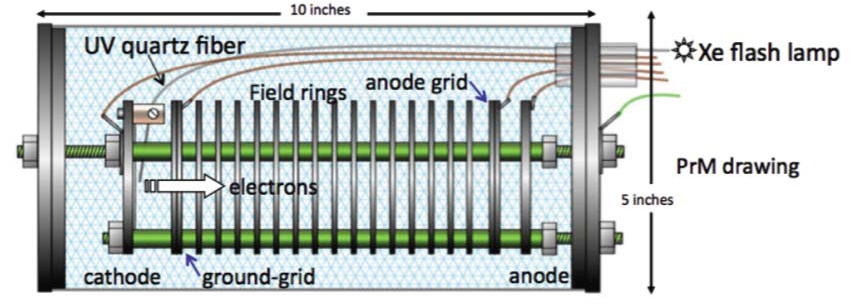
\includegraphics[height=3cm]{PrMon_prm.pdf}
%\caption{Schematic diagram of the basic purity monitor design~\cite{Adamowski}. [CITATION: M. Adamowski et al.,The Liquid Argon Purity Demonstrator, JINST 9, P07005 (2014).]}
%\label{fig:prm}
%\end{figure}
\begin{dunefigure}[Purity Monitor diag]{fig:prm}
  {Schematic diagram of the basic purity monitor design~\cite{Adamowski:2014daa}.}
  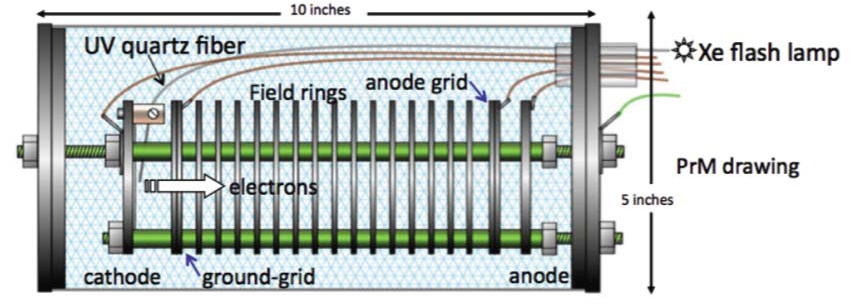
\includegraphics[width=0.5\textwidth]{PrMon_prm.pdf}
\end{dunefigure}

The photocathode that produces the photoelectrons is an aluminum plate coated with \SI{50}{\angstrom} of titanium and \SI{1000}{\angstrom} of gold and attached to the cathode disk. A xenon flash lamp is used as the light source in the baseline design, although this could potentially be replaced by a more reliable and possibly submersible light source in the future, perhaps LED driven. The UV output of the lamp is quite good around $\lambda=$ \SI{225}{\nano\meter}, which is close to the work function of gold (\SIrange{4.9}{5.1}{\eV}). Several UV quartz fibers are used to carry the xenon UV light into the cryostat to illuminate the gold photocathode.   Another quartz fiber is used to deliver the light into a properly biased photodiode outside of the cryostat to provide the trigger signal for when the lamp flashes. 

\subsubsection{Electronics, DAQ and Slow Controls Interfacing}
%Jianming
The purity monitor electronics and DAQ system consist of front-end electronics, waveform digitizers, and a DAQ PC.  The block diagram of the system is shown in Fig~\ref{fig:diag}. 

The baseline design of the front-end electronics is the one used for the purity monitors at the 35-ton detector, LBNF, and MicroBOONE. The cathode and anode signals are fed into two charge amplifiers contained within the purity monitor electronics module. This electronics module includes a HV filter circuit and an amplifier circuit that are shielded by copper plates, so the signal and high voltage can be carried on the same cable and decoupled inside the purity monitor electronics module. The amplified outputs of the anode and cathode will be recorded with a waveform digitizer that interfaces with a DAQ PC. The shields of the signal and HV cable connect to the grounding points of the cryostat and are separated from the electronic ground with a resistor and a capacitor connected in parallel, mitigating ground loops between the cryostat and the electronics racks. The amplified outputs are transmitted to an AlazarTech ATS310 waveform digitizer that contains two input channels each with 12-bit resolution. Each channel is capable of sampling a signal at a rate of \SI{20}{\mega\samples\per\second} to \SI{1}{\kilo\samples\per\second} and storing up to \SI{8}{\mega\samples} in memory. One digitizer is used per purity monitor and each interfaces with the DAQ PC across the PCI bus. 

%\begin{figure}[h]
%	\centering
%	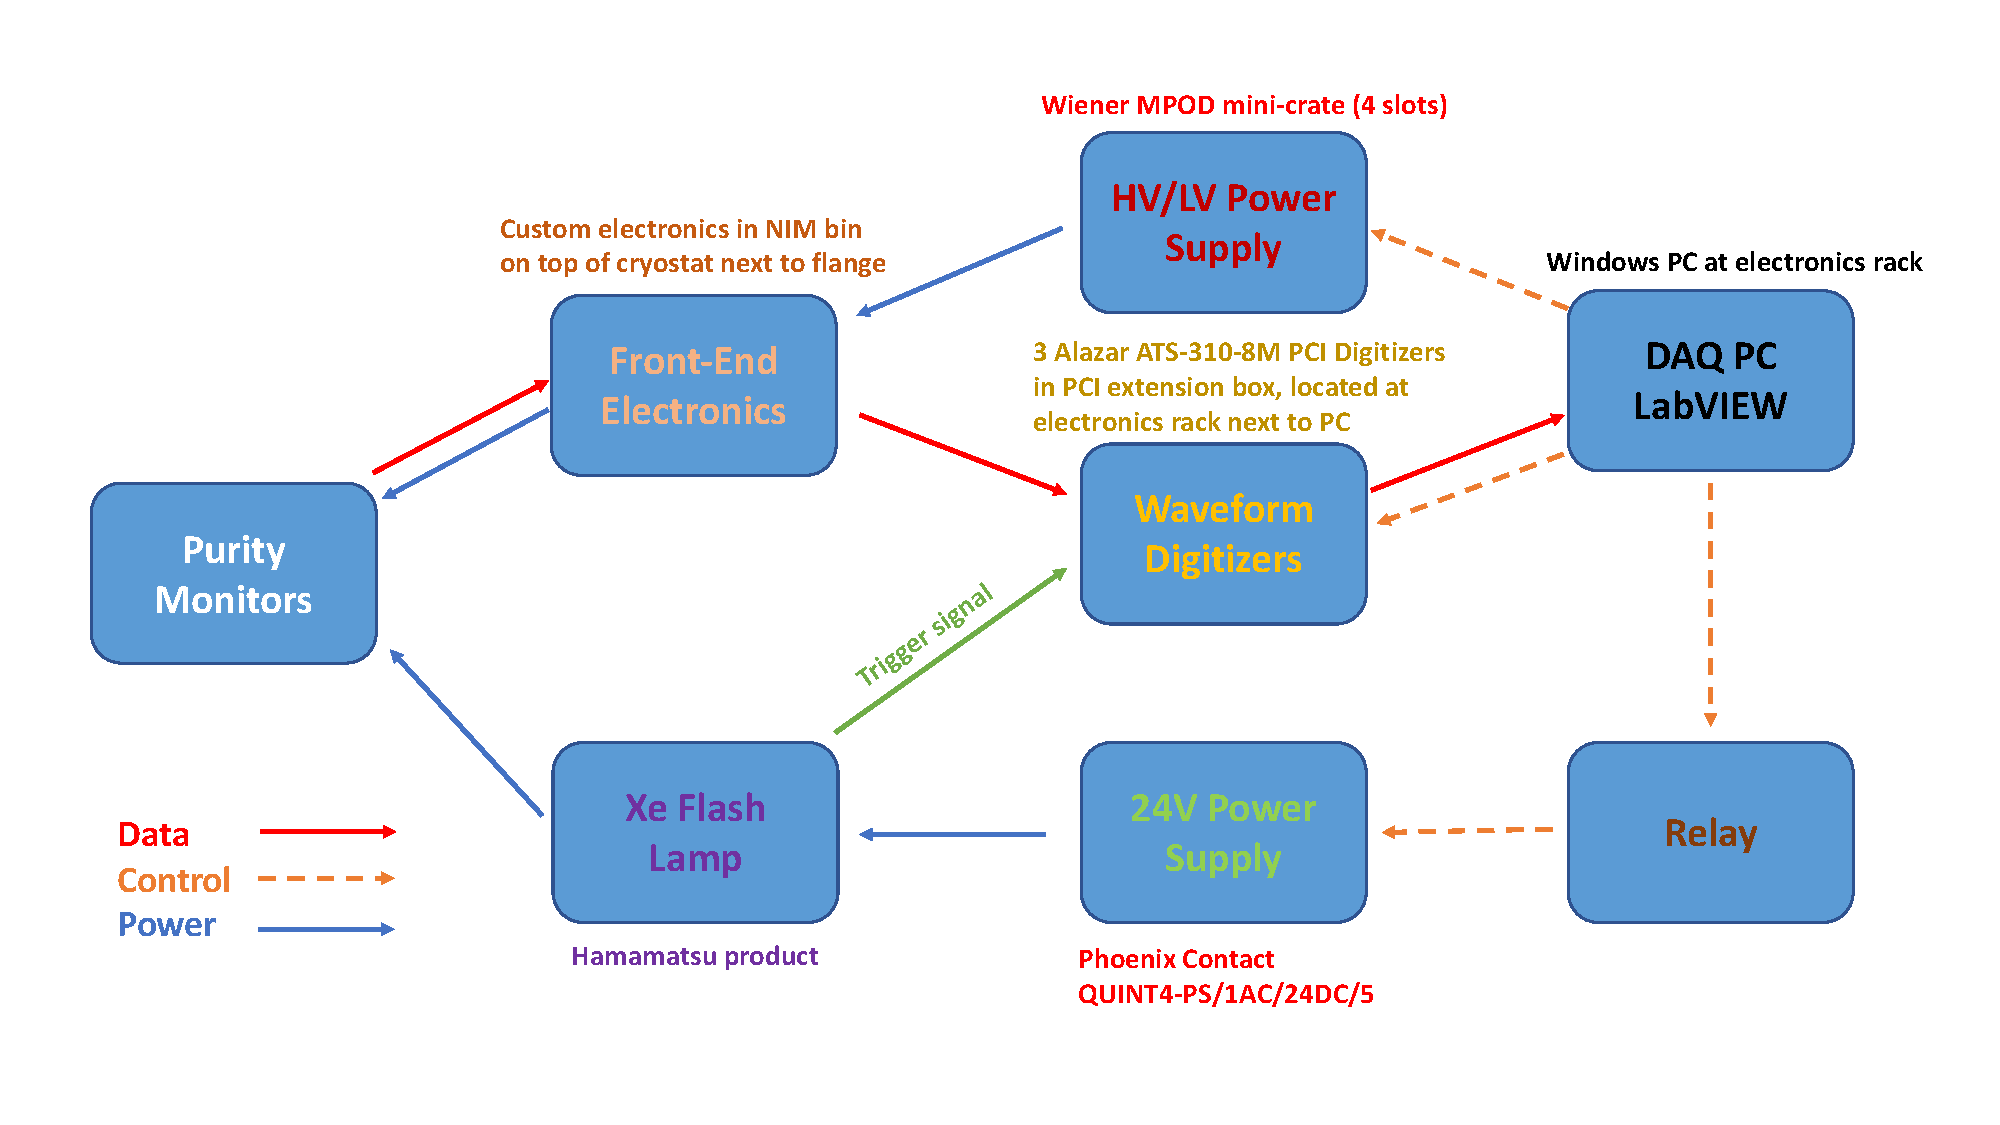
\includegraphics[width=0.8\textwidth]{PrMon_BlockDiagram.pdf}
%	\caption{Block diagram of the purity monitor system.}
%	\label{fig:diagram}
%\end{figure}
\begin{dunefigure}[Purity Monitor Block-diag]{fig:diag}
  {Block diagram of the purity monitor system.}
  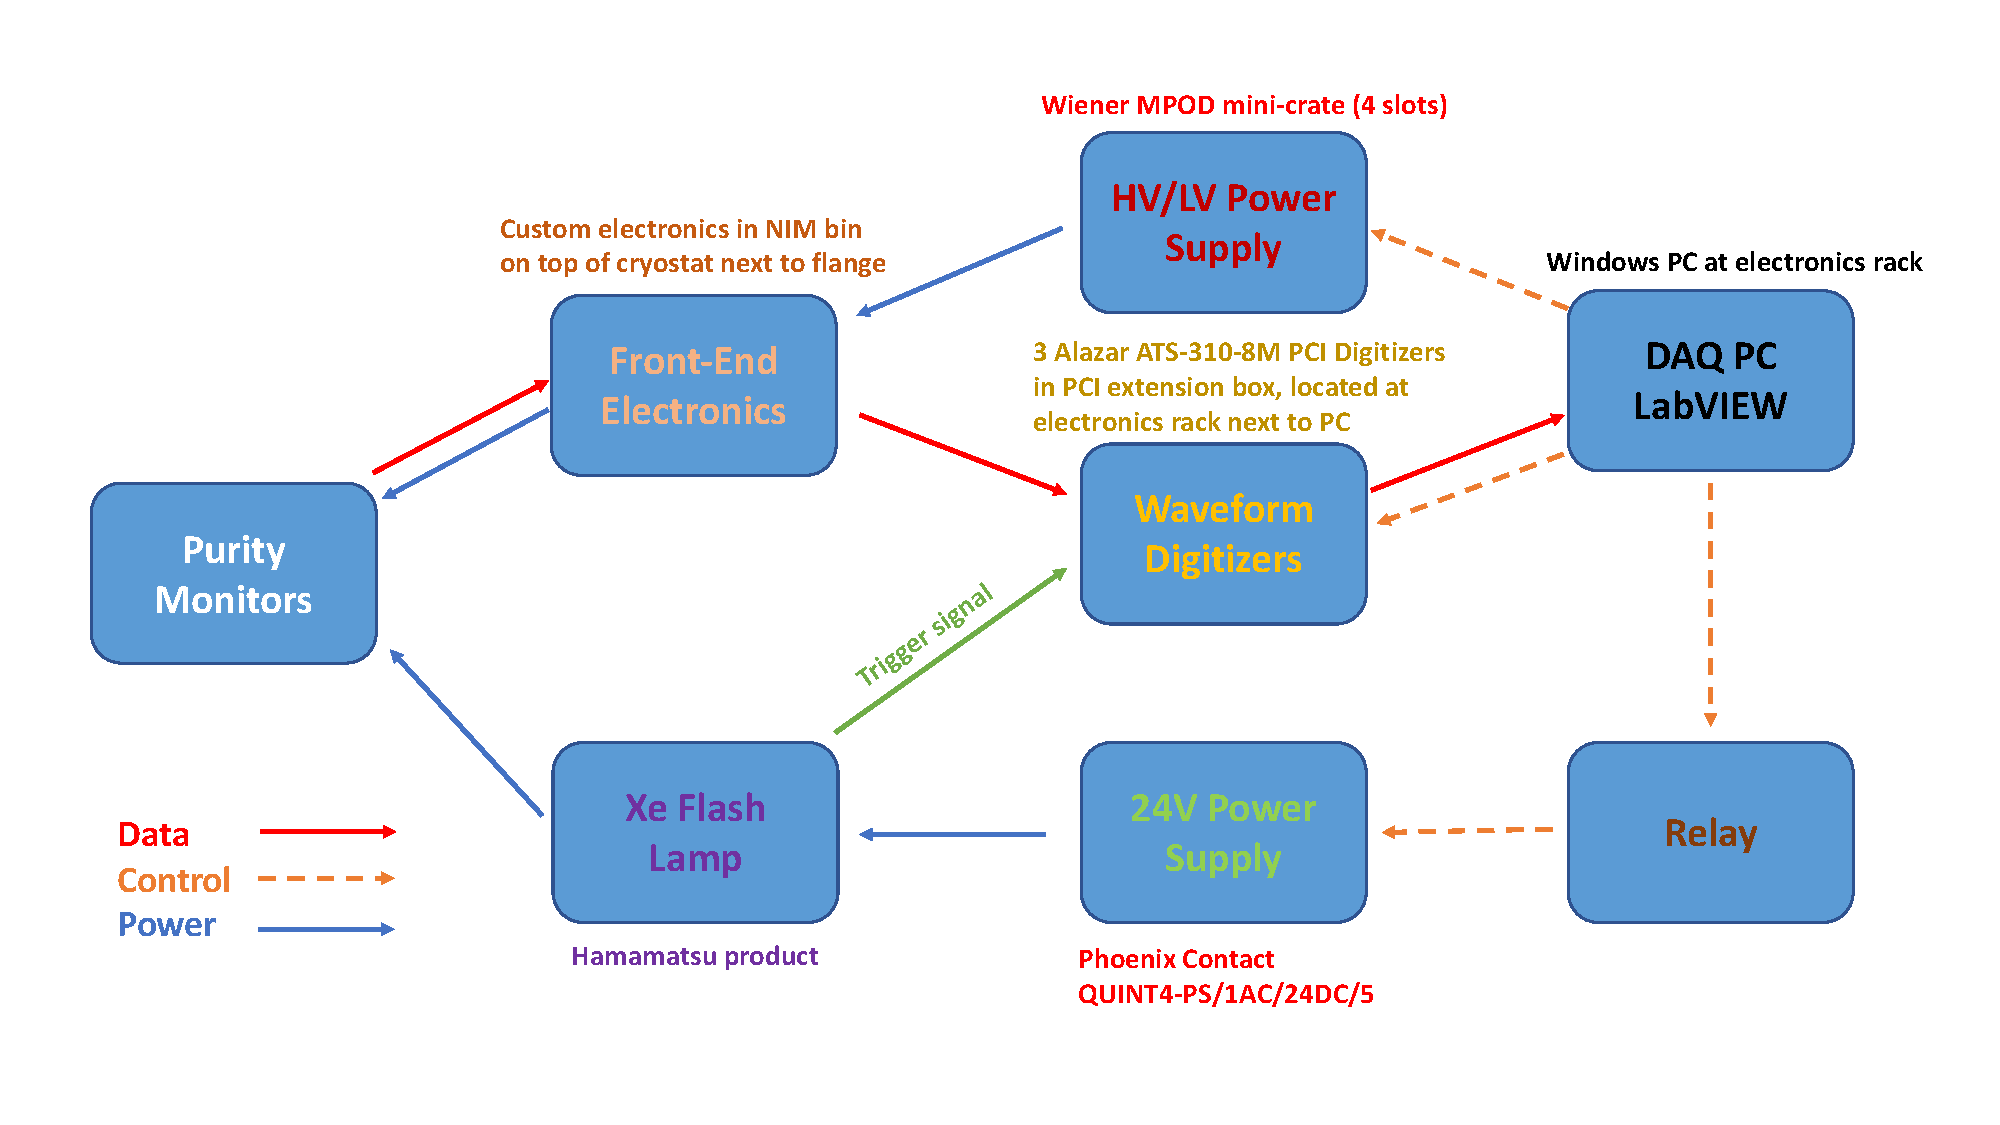
\includegraphics[width=0.5\textwidth]{PrMon_BlockDiagram.pdf}%
\end{dunefigure}

A custom LabVIEW application running on the DAQ PC is developed and consists of two functions: controlling the digitizers and the power supplies, and monitoring the signals and key parameters. The application configures the digitizers to set the sampling rate, the number of waveforms to be stored in the memory, pre-trigger data, and a trigger mode. A signal from a photodiode triggered by the xenon flash lamp is directly fed into the digitizer as an external trigger to initiate data acquisition. The LabVIEW application automatically turns on the xenon flash lamp by controlling powering a relay at the start of data taking and then turns it off when finished. The waveforms stored in the digitizers are transferred to the DAQ PC and used to obtain averaged waveforms in order to reduce the electronic noise present in waveforms. The baseline is estimated by using the pre-trigger data and subtracted from the waveforms to measure peak voltages of the cathode and anode signals. These processes are performed in real time within the application and are then used to estimate the electron lifetime. The application continuously displays the waveforms and important parameters, such as measured electron lifetime, peak voltages, and drift time of electrons in the purity monitors, as well as show these parameters over time. This allows one to validate the impurity of the LAr and see effects that may not be spotted at an instantaneous moment. Instead of storing the measured parameters, the waveforms and the digitizer configurations are recorded in binary form for offline analysis. ISEG HV modules in a WIENER MPOD mini crate are used to supply negative and positive voltages to the cathode and the anode, respectively. The LabVIEW application will control and monitor the HV systems through an Ethernet interface.  

The xenon flash lamp and the front-end electronics will be installed close to the purity monitor flange, to reduce light loss through the optical fiber and prevent signal loss. Other pieces of equipment will be mounted in a DCS rack separate from the cryostat. They distribute power to the xenon flash lamp and the front-end electronics, as well as collect data from the electronics. The DCS system will communicate with the purity monitor DAQ software and have control of the HV and LV power supplies of the purity monitor system. 

The electronics of purity monitors may induce noise in the TPC electronics, largely coming from the current surge in the discharging process of the main capacitor of the purity monitor xenon light source when producing a flash.  Although, this source of noise has largely been mitigated by placing the xenon flash lamp inside its own faraday cage allowing for proper grounding and shielding.  The light source for the purity monitor system will produce a lot of UV light in the detector which could potentially interfere with physics measurements and damage the Photon Detector System. To solve these problems, software will be developed for a light source triggering mechanism to prevent the purity monitor flash lamp from flashing during TPC and photon detector data taking. The purity monitor will also send signals to TPC and photodetectors to veto any TPC/photon signals during purity monitor measurements. 


\subsubsection{Production and Assembly}
\label{sec:PrMon-Production-Assembly}
%Andrew
Production of the individual purity monitors and the assembly of them into the string that will be placed into the DUNE-FD cryostat will follow the same methodology that is being developed for DUNE.  Each of the individual monitors will be fabricated, assembled and then tested in a smaller test stand.  After confirming that each of the individual purity monitors operates at the required performance, they would be assembled together via the support tubes used to mount the system to the inside of the cryostat such that three purity monitors are grouped together to form a "string" of purity monitors, as shown in Fig.~\ref{fig:PrMon-SystemString}.  The assembly of the individual purity monitors into the string would follow the steps laid out in the first 5 panels of Fig.~\ref{fig:PrMon-Assembly}.  Each monitor would be assembled as the string is built from the top down, and in the end there would be three individual purity monitors hanging from a single string.  The assembly of the string would conclude once the purity monitors were each in place, but with the faraday cages removed and the HV cables and optical fibers yet to be run.  This full string assembly would then be shipped to the DUNE-FD site for installation into the cryostat.

\begin{dunefigure}[Purity Monitor String]{fig:PrMon-SystemString}
  {Design of the purity monitor string that will contain three purity monitors.}
  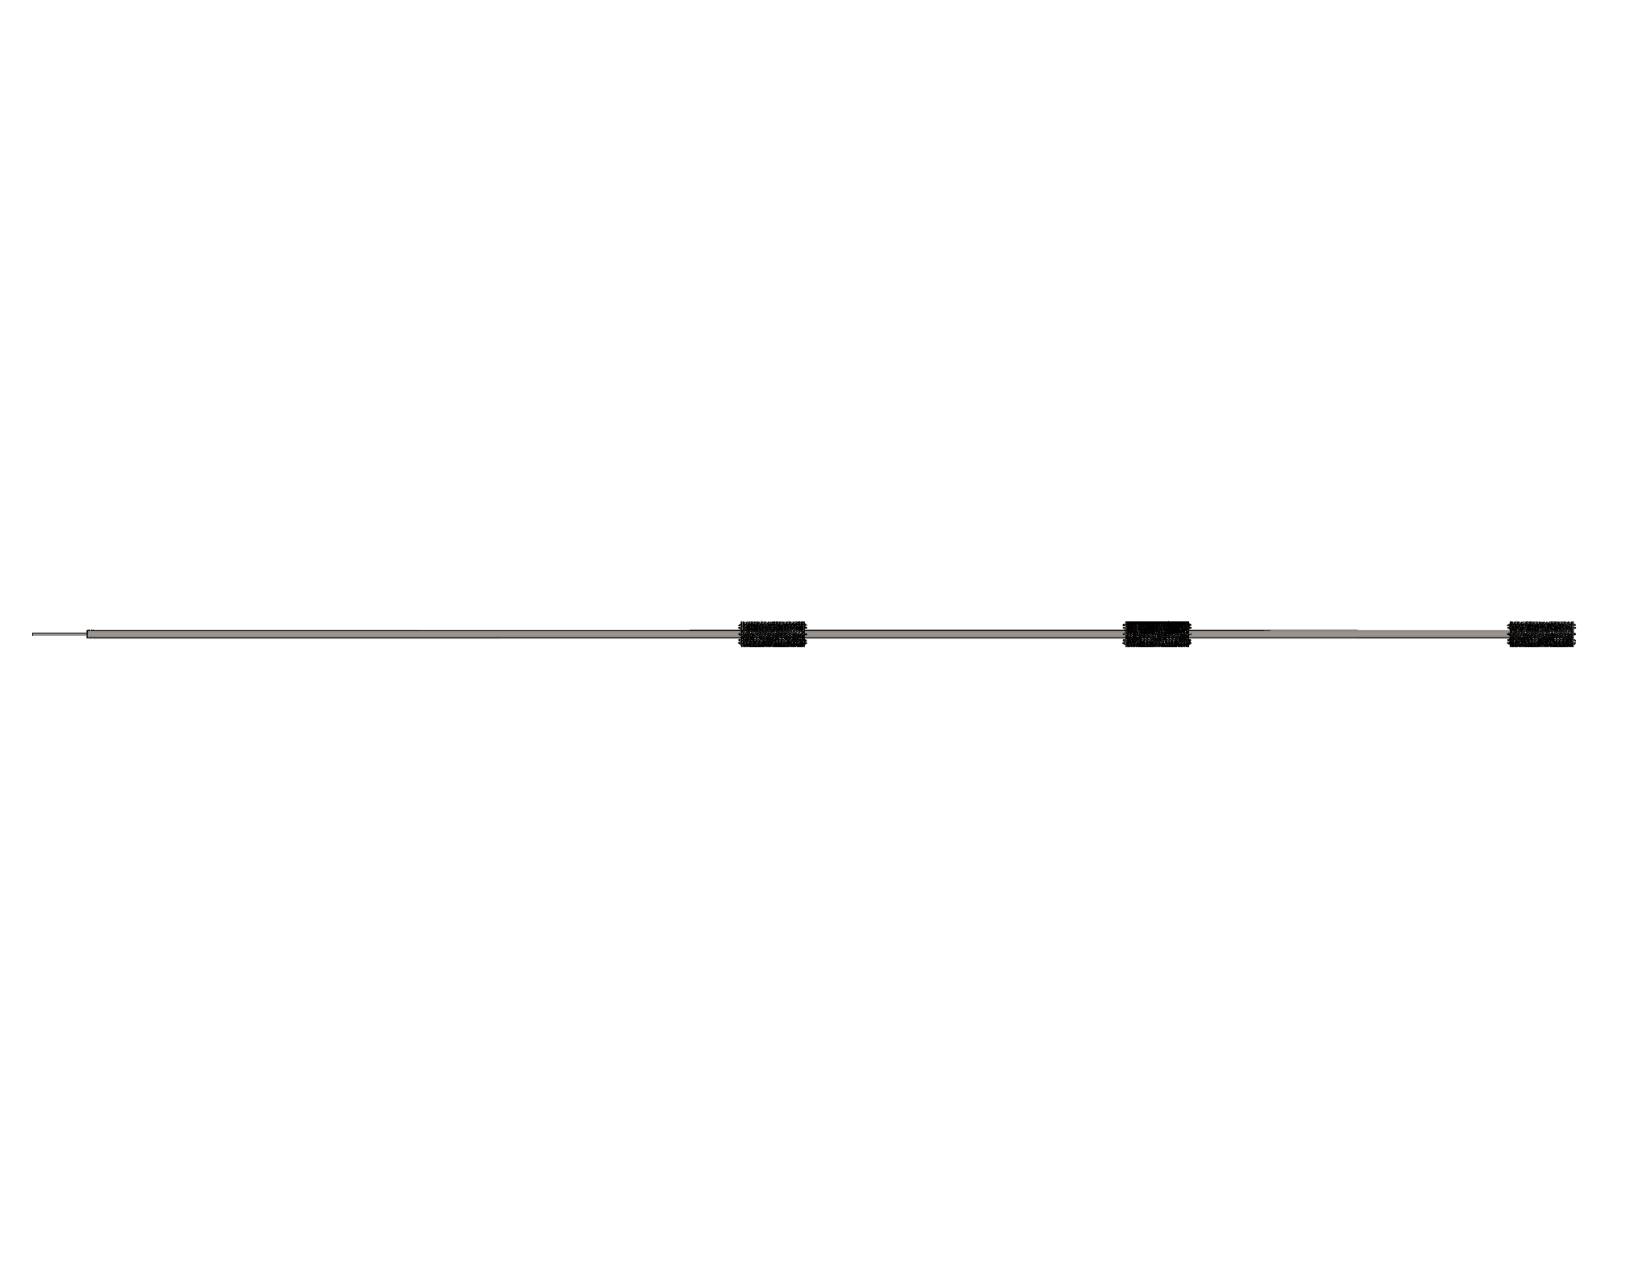
\includegraphics[width=\textwidth]{PrMon-SystemString.pdf}
\end{dunefigure}

\begin{dunefigure}[Purity Monitor String Assembly]{fig:PrMon-Assembly}
  {Assembly sequence of the purity monitors.}
  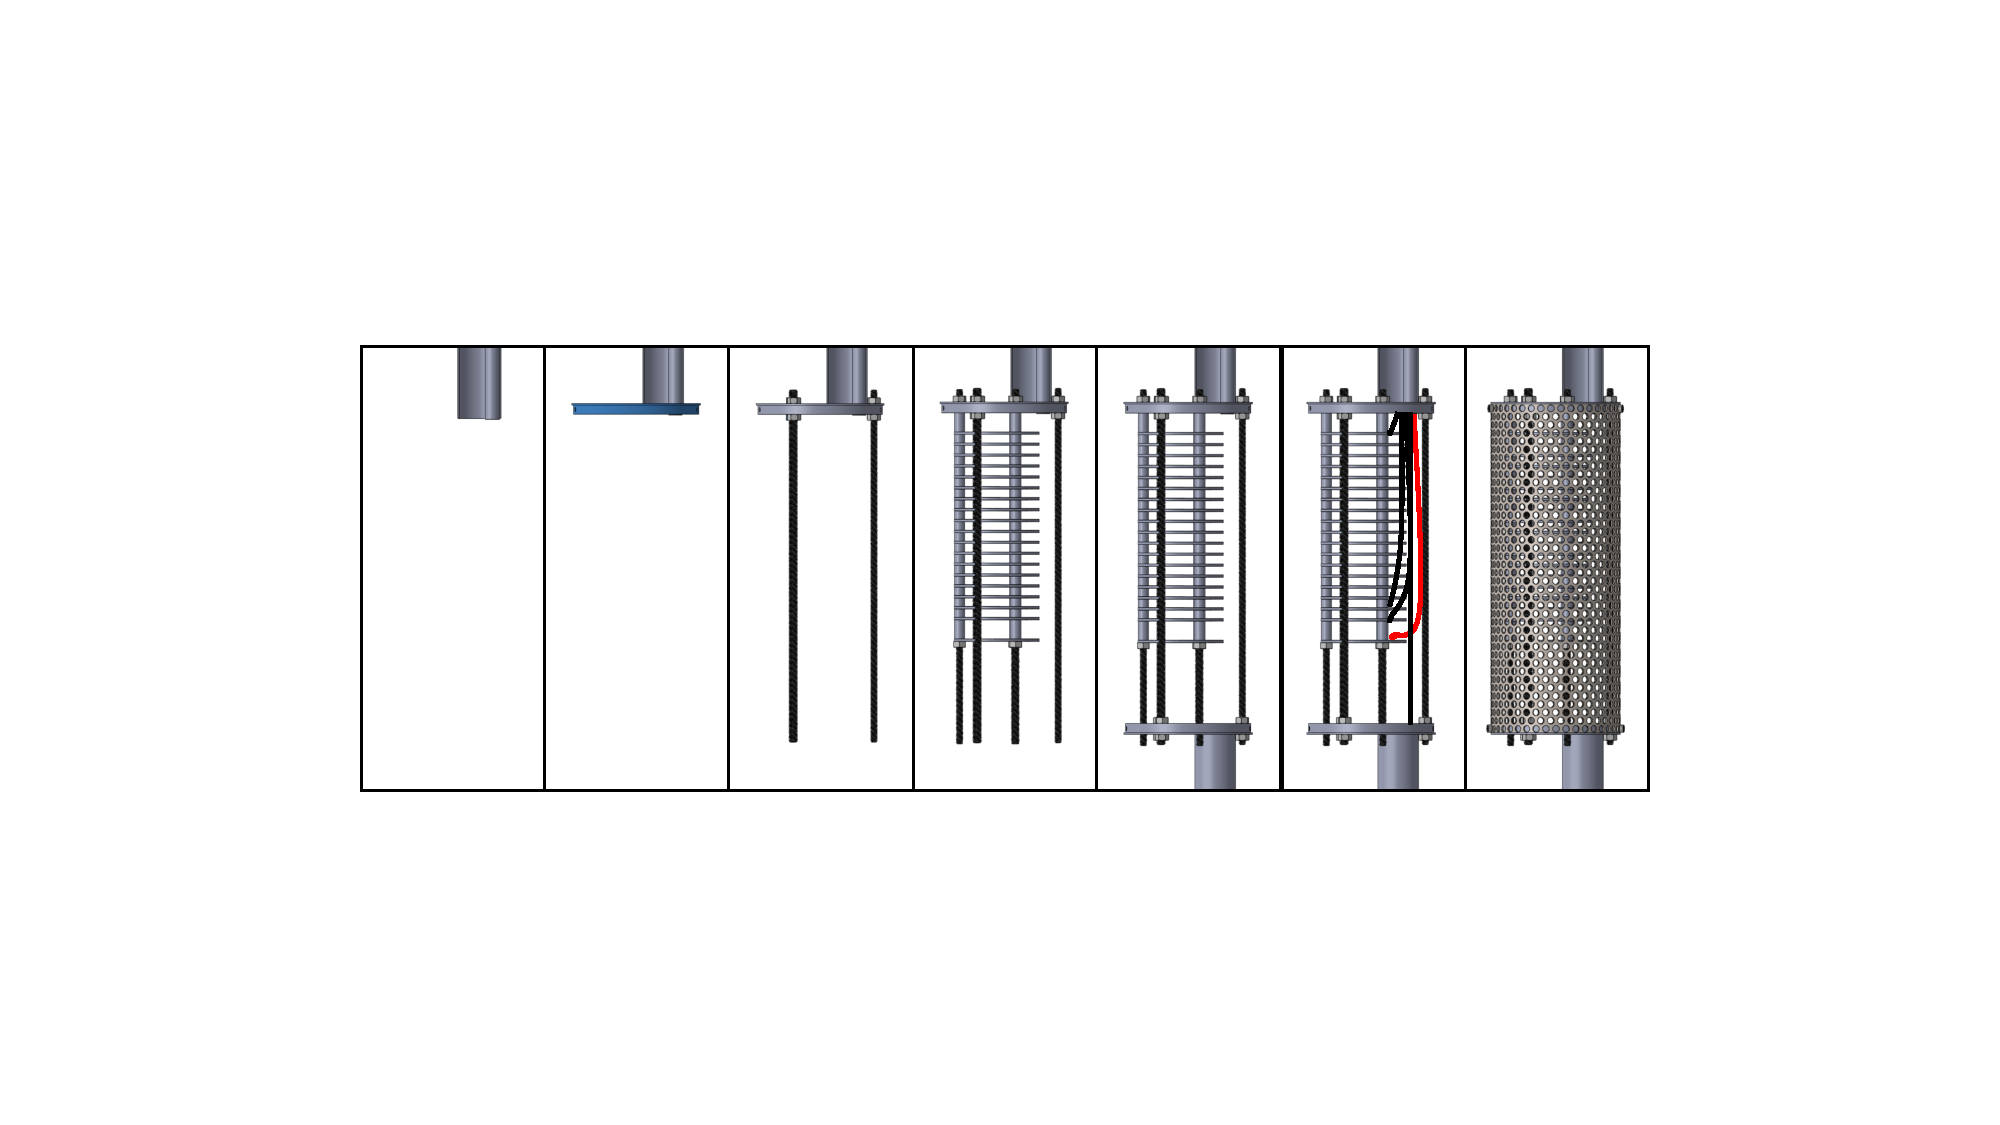
\includegraphics[width=\textwidth]{PrMon-Assembly.pdf}
\end{dunefigure}



